\problemname{KATT:s and rats}
\noindent
A special type of mutated giant rats have taken over the sewers of Gothenburg,
and the city management has asked for your help in solving the problem.

The sewer consists of $N$ manholes numbered from $1$ to $N$, with $N-1$ pipes connecting the manholes.
Each pipe connects two manholes, and the sewer is designed
so that it is possible to travel between each pair of manholes by going through a sequence of pipes.
To reduce costs, all sewer developers in Gothenburg have been fired,
leaving the sewer system completely undocumented.
This means that there is no one left who knows between which pairs of manholes there are pipes.

There are a total of $K$ mutated giant rats, located in different manholes.
As the rats are extremely large and aggressive, there can never be two rats in the same manhole.
You have already placed out $K$ KATT:s (Kinetically Activated Tripping Trap) in different manholes.
These can be activated with a single button press,
and you now want to try to get the rats to go to the manholes with the KATT:s.
But the rats are very intelligent, and if not all KATT:s are activated simultaneously, they will
learn to use the KATT:s against you.

To get the rats to move, you have a large number of OWL:s
(Omnidirectional Wave Launchers),
which play songs and make noises that are especially irritating to this type of mutated giant rats.
You can, in several rounds, choose a subset of the manholes, and place an OWL in each manhole in the subset.
In every round, you will place some OWL:s, and some rats might go through a pipe in order to escape the annoying sounds.
More specifically, each rat will get the opportunity to flee,
and due to the laws of physics, the rats will do this in the order of the number of the manhole they are in right now.
That is, if there are rats in manholes number $1$ and $2$, the rat in manhole $1$ will try to flee first.
When this rat has finished fleeing, the rat in manhole $2$ will perform its escape.
The rats want to maximize the distance to the nearest OWL.
A rat will consider moving to all manholes, free from other rats,
within one pipe's distance from where it is right now.
If none of these manholes have a strictly larger distance to the nearest OWL, the rat will stay where it is now.
Otherwise, it will move to the adjacent manhole with the greatest distance to the nearest OWL.
If there are multiple such manholes, the rat will choose the manhole with the lowest number amongst them.
The distance between two manholes is the minimum number of pipes you must go through to travel between them.

You have received a large number of OWL:s from the city of Gothenburg, but you can only make $25000$ rounds of placements of OWL:s before
the mating season of giant mutated rats begins (which would have disastrous consequences!).

\section*{Interaction}
First, your program should read the numbers $N$ ($2 \leq N \leq 100$) and $K$ ($1 \leq K < N$), which are written on a line.
Then follows a line with $K$ different numbers $1 \leq r_1 < ... < r_K \leq N$, describing the numbers of the manholes where the rats are initially located.
After that, a line with $K$ different numbers $1 \leq t_1 < ... < t_K \leq N$ is given, describing the numbers of the manholes where there are KATT:s.

When you want to make a placement of OWL:s, you should first write out a number $M$, the number of OWL:s you are placing out.
Then you should, on the same line, write out the numbers $1 \leq s_1 < ... < s_M \leq N$,
the manholes where you want to place OWL:s. OWL:s can be placed in a manhole regardless of whether there is a rat there or not.
Then your program should read a line with $K$ numbers, $1 \leq r_1 < ... < r_K \leq N$,
the manholes where there are rats after all rats have tried to flee from the sound.

When you have managed to get all rats to manholes with KATT:s, you should write out ``\texttt{activate!}'' on a line.
Your program should then terminate.

\textbf{Make sure to flush the output after each query}, otherwise you may get a \textit{Time Limit Exceeded}.
In C++, this can be done for example with \texttt{cout << flush;}
or \texttt{fflush(stdout);},
in Python with \texttt{stdout.flush()}
and in Java with \texttt{System.out.flush();}.
The sewer is not necessarily randomly generated.
However, it is guaranteed that rats start at and KATT:s are placed in manholes uniformly at random.
The judge is not adaptive, which means it is predetermined what the sewer§ looks like.

To facilitate the testing of your solution, we provide a simple tool that you can download. See ``attachments''
at the bottom of the Kattis problem page. Refer to the comment at the top of the file for a description of how it can be used.

\section*{Scoring}
Your solution will be tested on a set of test case groups.
To get points for a group, you must pass all the test cases in the group.

\noindent
\begin{tabular}{| l | l | l |}
\hline

\textbf{Group} & \textbf{Point value} & \textbf{Constraints} \\ \hline \hline
$1$ & $5$ & $N = 2$ \\ \hline
$2$ & $5$ & $N \leq 3$ \\ \hline
$3$ & $9$ & $N \leq 10$ \\ \hline
$4$ & $20$ & $K = 1$ \\ \hline
$5$ & $15$ & There is a pipe between manhole $i$ and manhole $i+1$ for all $1 \leq i < N$. \\ \hline
$6$ & $21$ & $N \leq 50$ \\ \hline
$7$ & $25$ & No additional constraints. \\ \hline

\end{tabular}

\section*{Explanation of sample case 2}

\begin{centering}
  \begin{figure}[h]
    \centering
    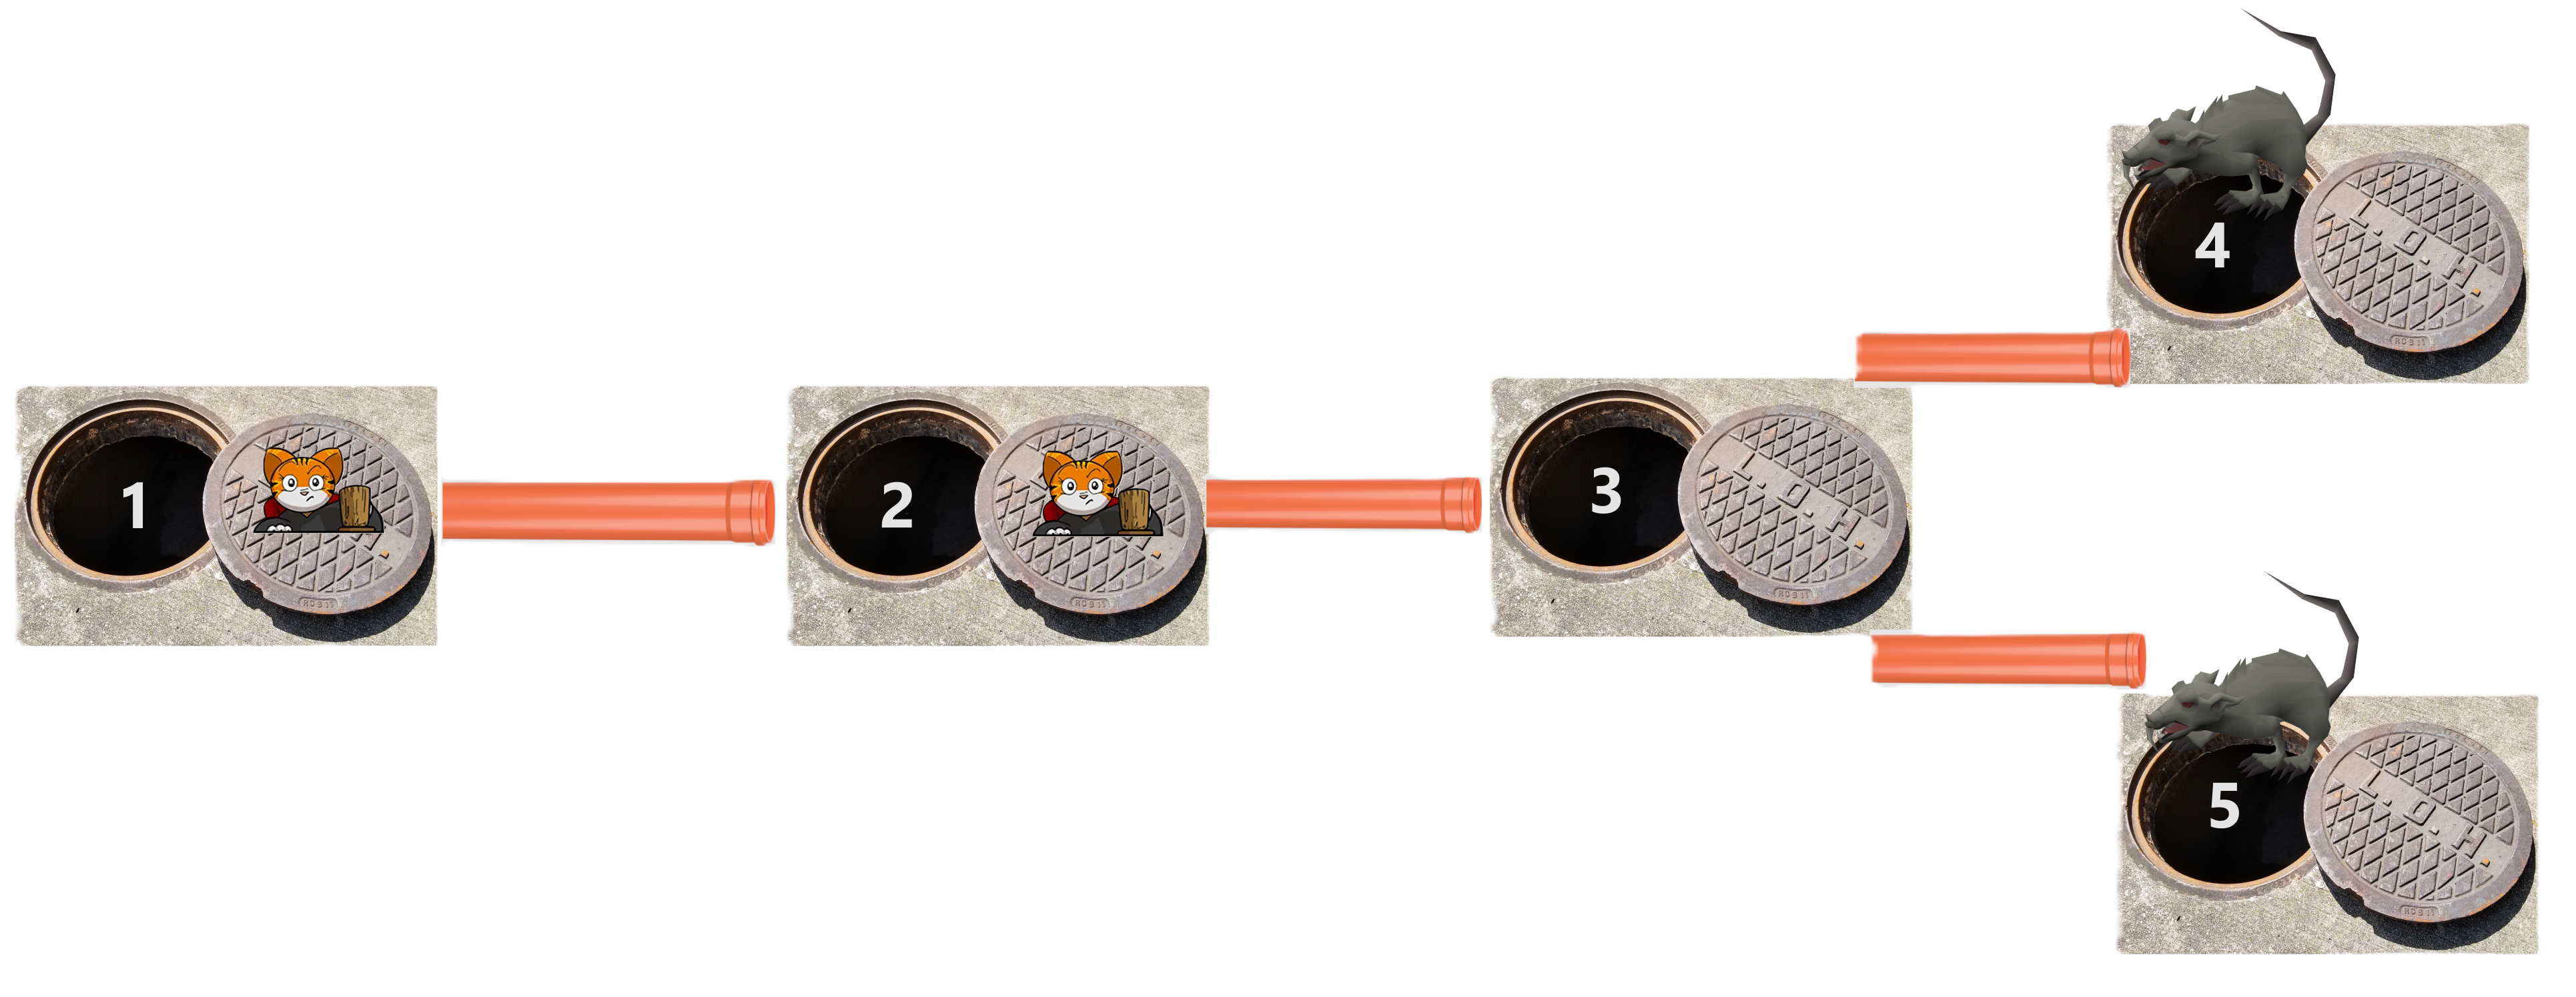
\includegraphics[scale=0.2]{rats_graph before.png}
    \caption{The layout of the sewer in sample 2. Note that your program will not know the layout of the pipes.}
  \end{figure}
\end{centering}

\begin{centering}
  \begin{figure}[h]
    \centering
    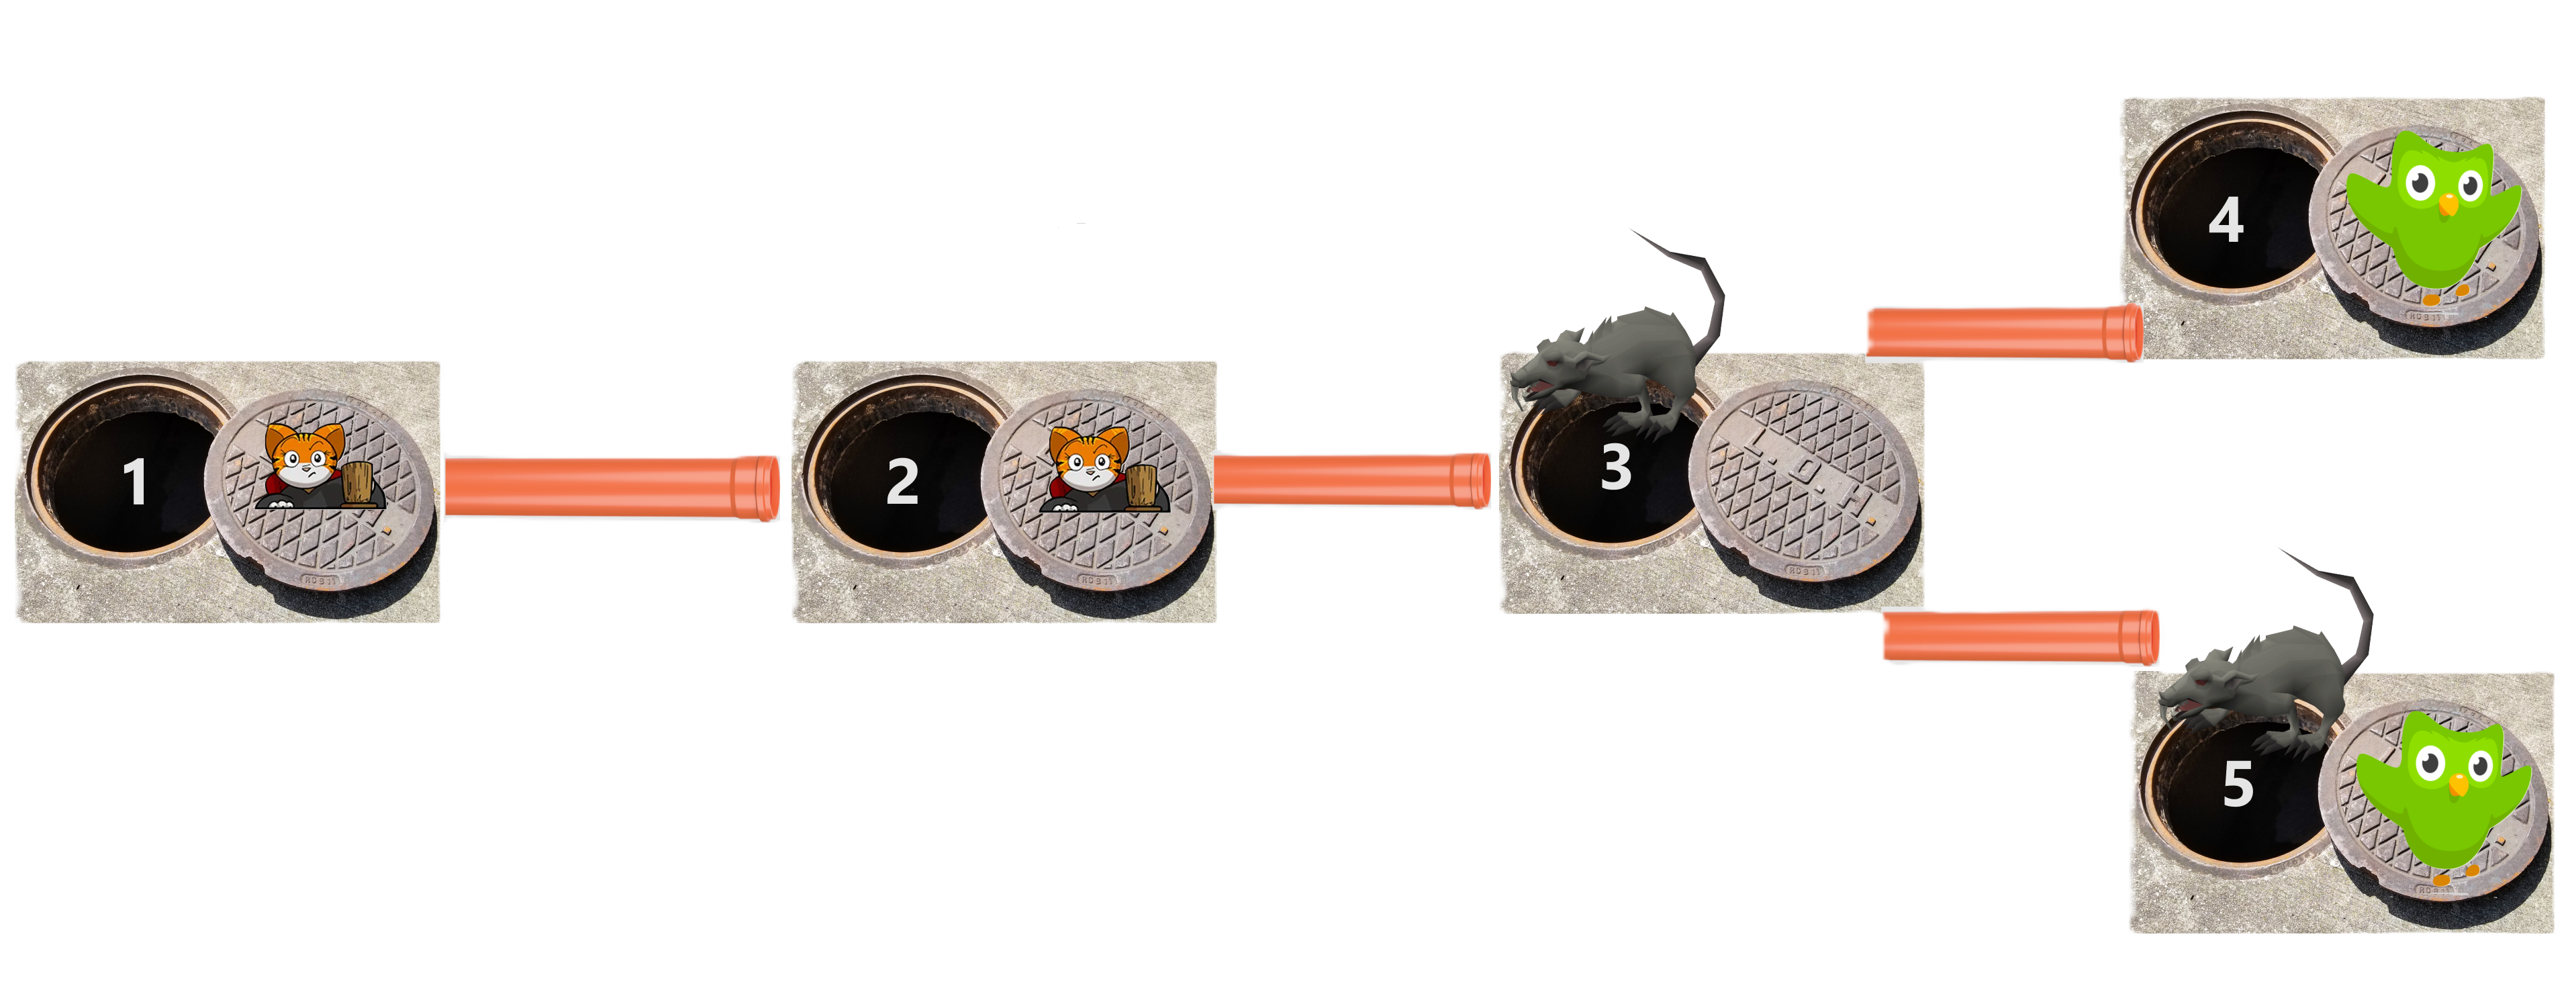
\includegraphics[scale=0.2]{rats_graph step1.png}
    \caption{When you place OWL:s in manholes 4 and 5, the rats will be very disturbed. Firstly, the rat in manhole 4 will try to escape, since $4 < 5$. This rat will go to manhole 3. After this, the rat in manhole 5 tries to escape, but has no available manhole to go to.}
  \end{figure}
\end{centering}

\begin{centering}
  \begin{figure}[h]
    \centering
    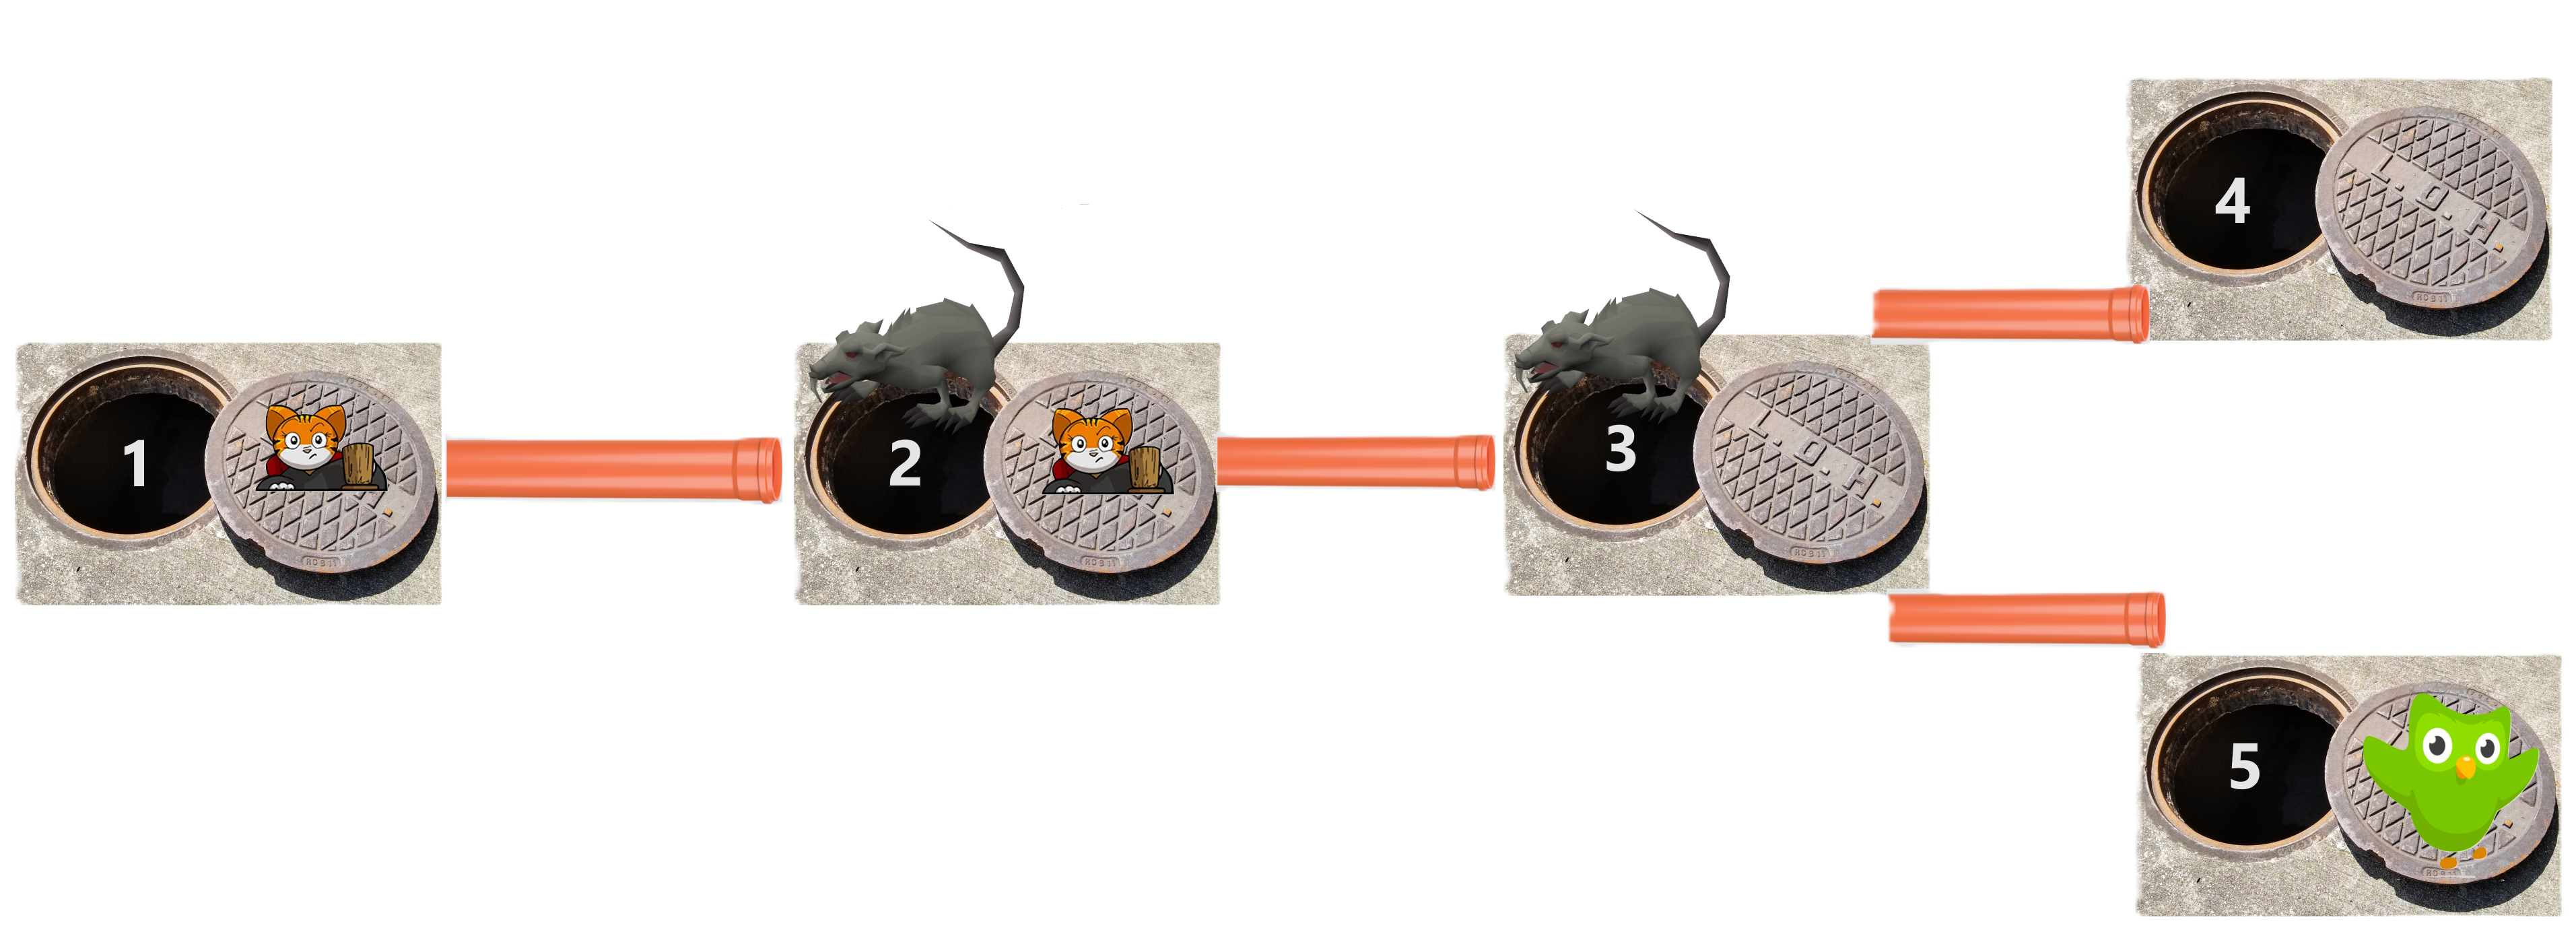
\includegraphics[scale=0.2]{rats_graph step2.png}
    \caption{When you place a single OWL in manhole 5, first the rat in manhole 3 flees to manhole 2, and then the rat in manhole 5 flees to manhole 3.}
  \end{figure}
\end{centering}

\begin{centering}
  \begin{figure}[h]
    \centering
    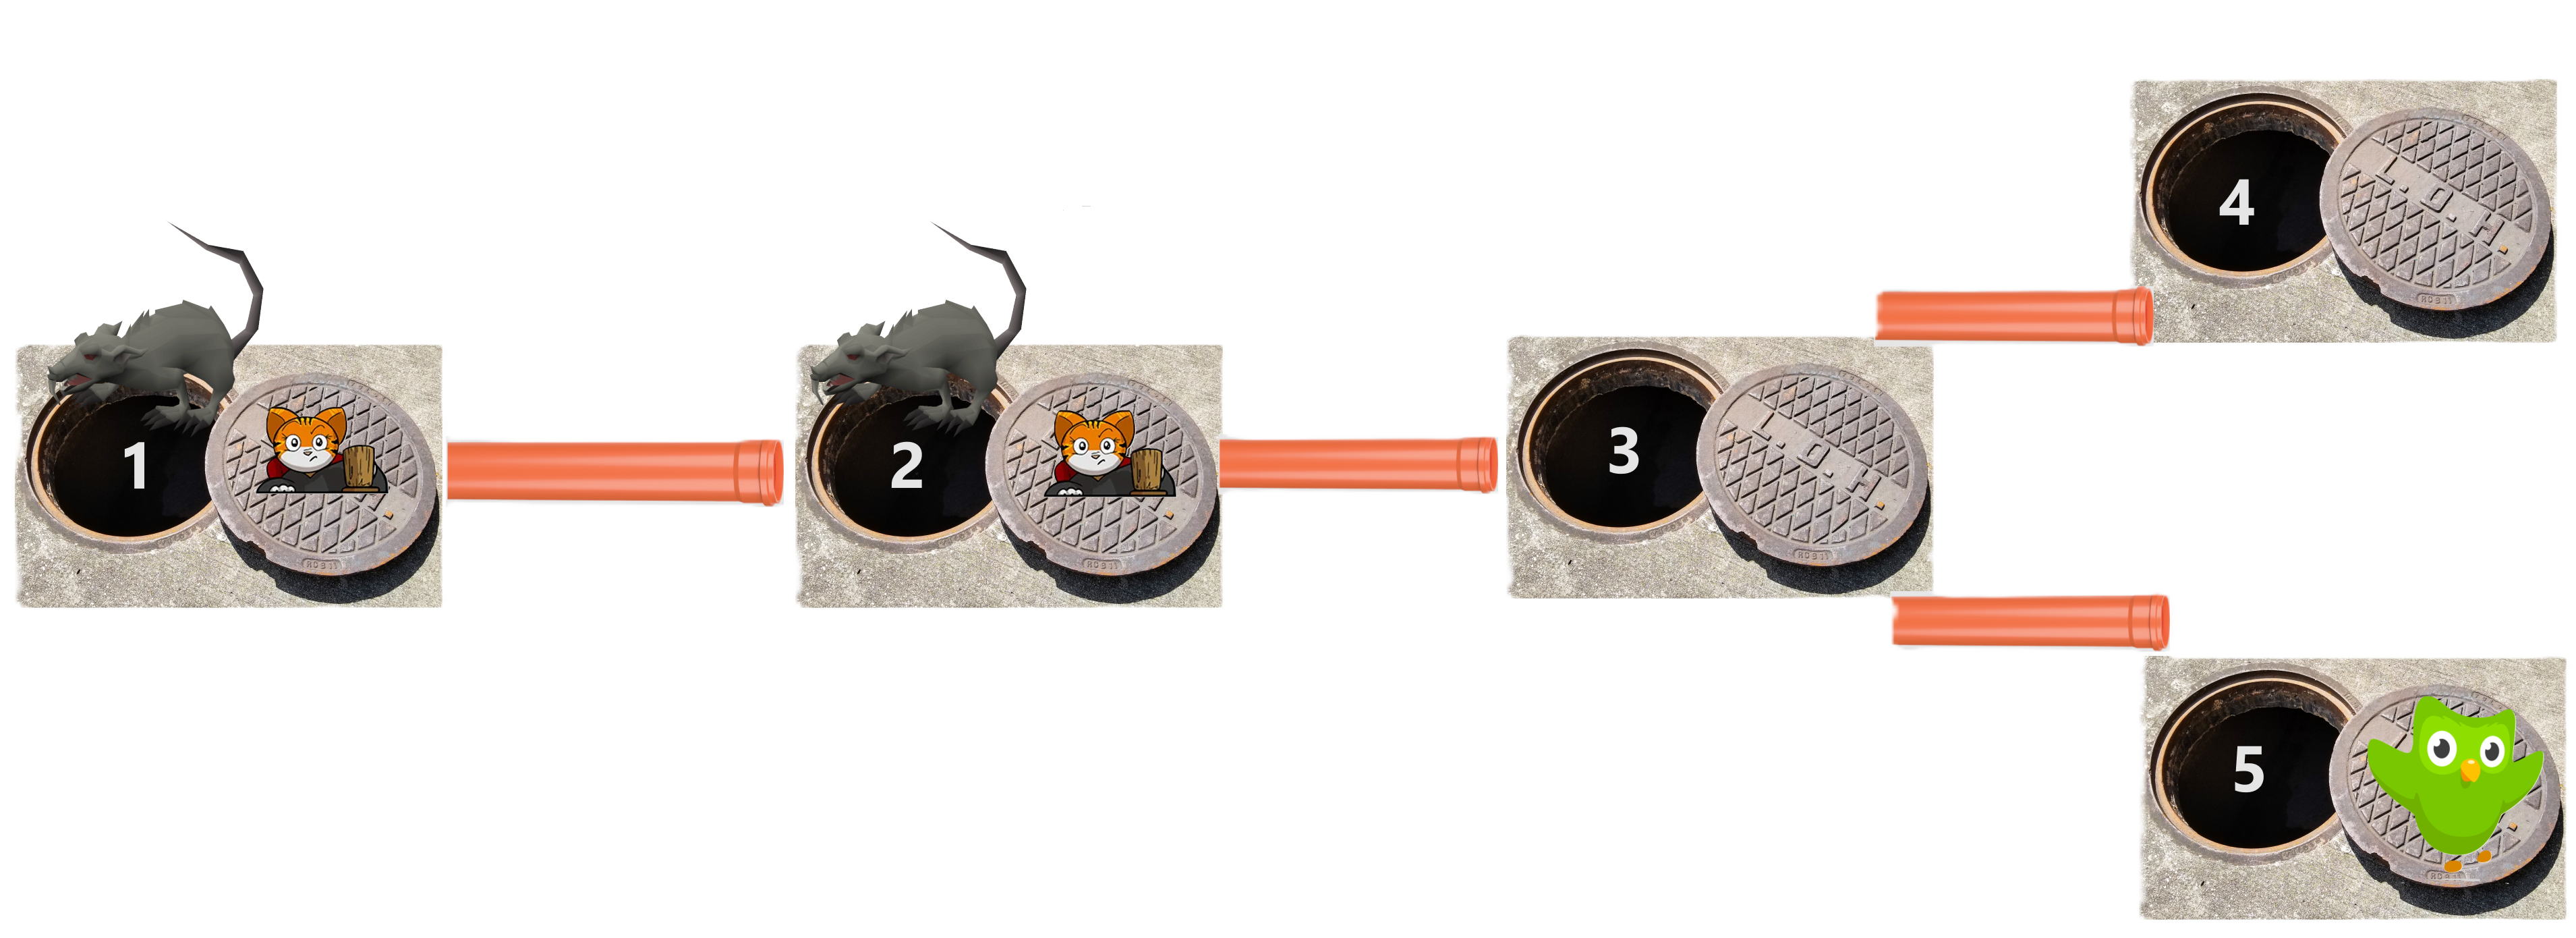
\includegraphics[scale=0.2]{rats_graph step3.png}
    \caption{When you once again place a single OWL in manhole 5, first the rat in manhole 2 flees to manhole 1, and then the rat in manhole 3 flees to manhole 2.}
  \end{figure}
\end{centering}

\begin{centering}
  \begin{figure}[h]
    \centering
    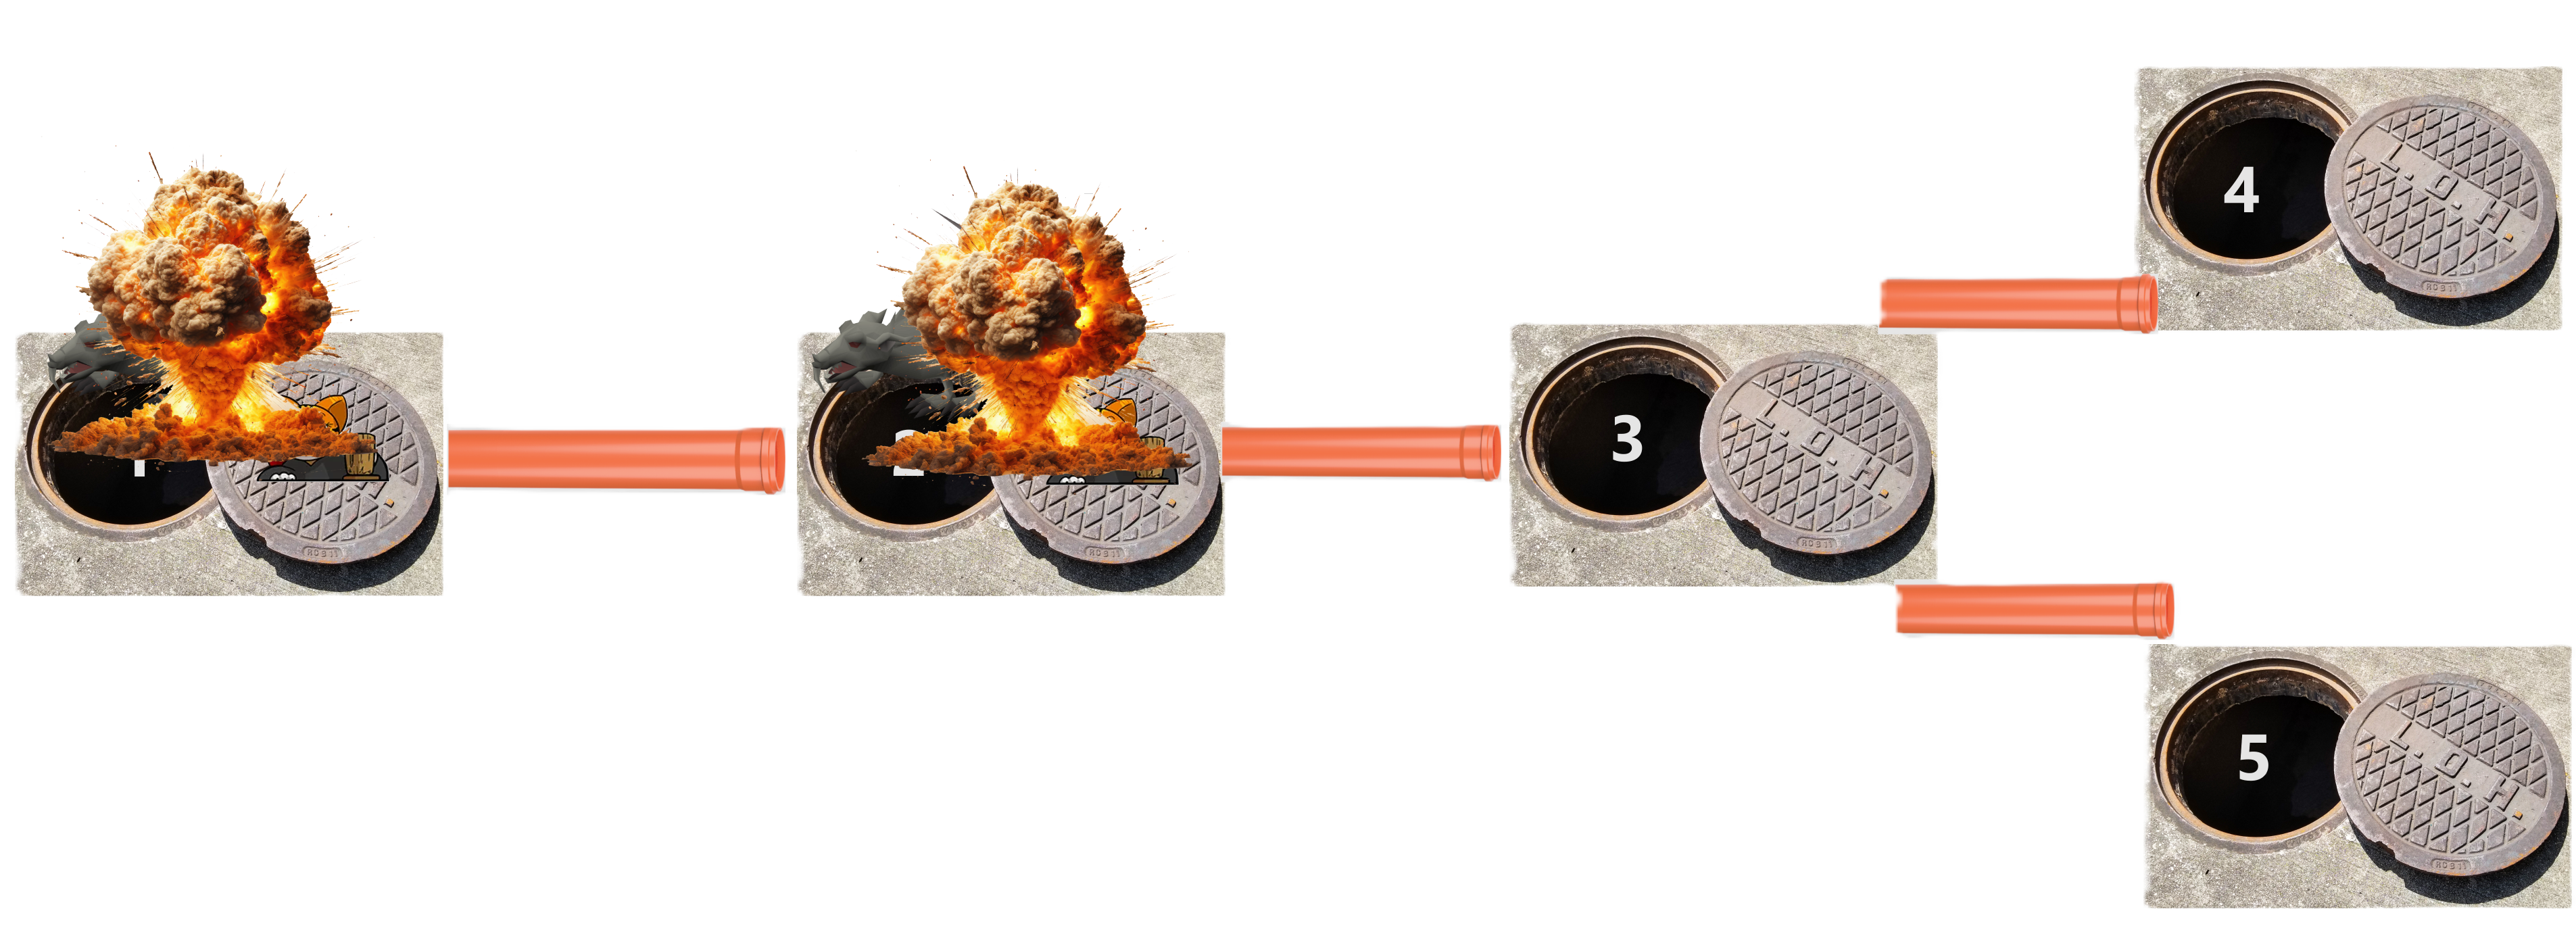
\includegraphics[scale=0.2]{rats_graph step4 activate.png}
    \caption{Now all rats are in manholes with KATT:s, and you can thus activate the KATT:s.}
  \end{figure}
\end{centering}

